\documentclass[fr]{../../../../../../eplexam}
\usepackage{../../../info-FSAB1402-exam}
\usepackage{../../../../../../eplcode}
\usepackage{listings}

\hypertitle{info-FSAB1402}{3}{FSAB}{1402}{2016}{Janvier}
{Martin Braquet \and Jean-Martin Vlaeminck}
{Peter Van Roy}

\lstset{
	language=Oz,
	breaklines=true,
	breakatwhitespace=true,
	%escapeinside={\%}{*)},
}

\section{Programmation fonctionnelle ( /4)}

Suivez les instructions suivantes :

\begin{itemize}

\item  Supposez deux matrices représentées en liste de listes
$$P = [[p_{11} \ldots p_{1b}][p_{21} \ldots p_{2 b}] \ldots [p_{a 1}\ldots p_{ab}]]$$
$$Q = [[q_{11} \ldots q_{1 n}][q_{21} \ldots q_{2 n}]\ldots [q_{m 1} \ldots q_{mn}]]$$
La taille de $P$ est (a x b) et la taille de $Q$ est (m x n). Nous supposons que $a \leq m$ et $b \leq n$.
Les éléments $p_{ij}$ et $q_{ij}$ ont la valeur 0 ou 1. Chaque valeur 1 représente un carré et chaque valeur 0
représente un vide. $P$ représente une figure connexe que l’on appelle un polyomino. $Q$ représente une figure
pas forcément connexe qui contient un certain nombre de carrés répartis dans un rectangle de taille (m x n).

Par exemple :
$$P = [[1\: 0\: 0][1 \:0\: 0][1\: 1\: 1]]$$
$$Q = [[1 \:0 \:0 \:1][0 \:0 \:1 \:0][0\: 1 \:0 \:0]]$$
représente
\begin{figure}[h]
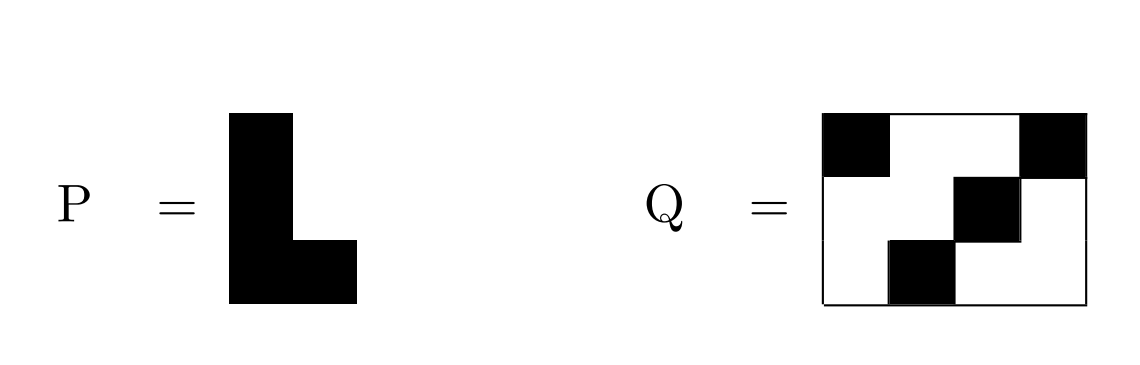
\includegraphics[width=\columnwidth]{PQ.png}
\end{figure}

\item Définissez la fonction \lstinline|{Match P Q}| qui renvoie \lstinline|yes| si $P$ peut se caser dans le coin supérieur gauche de $Q$
et \lstinline|no| sinon. C’est à dire, pour chaque élément $p_{ij}$ de $P$ qui est 1, l’élément correspondant de $Q$ est 0.
Pour les deux figures illustrées ci-dessus, \lstinline|{Match P Q}| = \lstinline|no|.
\item Définissez la fonction \lstinline|{Find P Q}| qui renvoie \lstinline|found(I J)| si P peut se caser quelque part dans Q et le coin
supérieur gauche de $P$ se trouve à la rangée $I$ et la colonne $J$ de $Q$. S’il n’y a pas de possibilités de caser $P$
complètement à l’intérieur du rectangle $Q$, alors la fonction renvoie \lstinline|notfound|.

\end{itemize}

Définissez \lstinline|Match| et \lstinline|Find| en utilisant uniquement des fonctions récursives terminales et déclaratives. Attention à utiliser une fonction par boucle. C’est à dire, pour traverser toutes les cases de $P$ ( ou de $Q$) il faut deux
fonctions récursives terminales. Attention à donner une spécification pour chaque fonction auxiliaire que vous
définissez.

\begin{solution}

\lstinputlisting{Janvier-2016-Q1.oz}

\end{solution}

\section{Sémantique ( /5))}
Voici un petit programme:

\lstinputlisting{Q2.oz}

Répondez aux question suivantes:
\begin{itemize}

	\item Qu'est-ce qui est affiché quand on exécute ce programme ? ( /0,5)

	\item Donnez la traduction de ce programme en langage noyau. Attention à donner une traduction complète ! ( /1)

	\item Donnez les environnements contextuels des procédures dans cette traduction. ( /0,5)

	\item Donnez quelques pas d'exécution de la machine abstraite pour bien montrer les choses suivantes:

 \begin{itemize}
 \item La création ( /0,5) et l'affectation ( /1) d'une cellule.

	\item La définition ( /0,5) et l'appel ( /1) d'une procédure.
 \end{itemize}

\end{itemize}

Attention à ne pas faire plus d'un pas d'exécution dans la machine abstraite pour chacun des 4 cas demandés.

\begin{solution}

\begin{itemize}
\item Il affiche 2.

\item \lstinputlisting{Q2-sol.oz}

\item
\[ CE_f=\{\texttt{C} \rightarrow c\} \]
\[ CE_{r3}=\{\texttt{C} \rightarrow c, \texttt{A} \rightarrow i7\} \]
\[ CE_{p1}=\{\texttt{C} \rightarrow c\} \]

\item
Toute l'exécution de la machine abstraite est effectuée ici, certains pas étant fusionnés s'ils n'apportent rien. Les états d'exécution à fournir à l'examen sont signalés ci-dessous. Parfois, il y a le choix entre plusieurs exemples de pas d'exécution : trouvez un juste milieu entre rapidité à obtenir (peu de pas depuis le début) et exhaustivité (beaucoup de choses à dire). On définit également, pour deux environnements $A$ et $B$, l'adjonction $A+B$ de la manière suivante:
\begin{itemize}
	\item Pour chaque identificateur commun aux deux ensembles, l'ensemble $A+B$ contient le mapping lié à l'identificateur de $B$.
	\item Pour les autres identificateurs, ils se retrouvent tous tels quels dans $A+B$.
\end{itemize}
Il s'agit d'une union avec remplacement des anciennes valeurs ($A$) par des nouvelles ($B$). Le concept s'étend aussi aux \emph{store} $\sigma_A$ et $\sigma_B$.

\begin{enumerate}
	\newcommand{\procc}[1]{\text{proc \{\$ #1\}}}
	\newcommand{\End}{\text{end}}
    \item
    \[ \Big([(<l1-l26>,E_0=\{ \texttt{Browse} \rightarrow browse, \texttt{NewCell} \rightarrow newcell \})],\]
    \[ \sigma_1=\{ browse=(\procc{A} \dots \End, CE_{browse}), newcell=(\procc{I C} \dots \End, CE_{newcell}) \}, \emptyset \Big) \]

    \item \emph{Avant la création d'une cellule}
    \[ \Big( [(<l2>, E_1 = E_0+\{C\rightarrow c, F\rightarrow f, P1\rightarrow p1, R3\rightarrow r3, R4\rightarrow r4, A1\rightarrow a1, I7\rightarrow i7\}), (<l3-l25>, E_1)], \]
    \[\sigma_2 = \sigma_1+\{c, f, p1, r3, r4, a1=0, i7\}, \emptyset \Big) \]
    Exécution du local. Composition. Création de valeur avec l'affectation de $0$ à $a1$. Composition.

    \item \emph{Après la création d'une cellule}
    \[ \Big([(<l3-l25>, E_1)], \sigma_2 +\{ c=\xi \}, \mu_1=\{c:a1\} \Big) \]

    \item \emph{Avant la définition d'une procédure}
    \[ \Big([(<l3-l12>, E_1), (<l13-l25>, E_1)],\sigma_2, \mu_1 \Big) \]
    Composition.

    \item \emph{Après la définition d'une procédure}
    \[ \Big([(<l13-l25>, E_1)], \sigma_3 = \sigma_2 + \{ f=(\procc{A R} <l4-l11> \End, CE_f) \}, \mu_1 \Big) \]
    Définition de la procédure $f$, et capture dans l'environnement contextuel de $\texttt{C} \rightarrow c$.

    \item Avant la définition de la procédure $p1$
    \[ \Big([(<l13-l21>, E_1), (<l22-l25>, E_1)], \sigma_3, \mu_1 \Big) \]
    Composition

    \item Après la définition de la procédure $p1$
    \[ \Big([(<l22-l25>, E_1)], \sigma_4 = \sigma_3 + \{ p1=(\procc{R5} <l14-l20> \End, CE_{p1}) \}, \mu_1 \Big) \]
    Il y a aussi capture de $\texttt{C}\rightarrow c$ dans l'environnement contextuel.

    \item \emph{Avant l'appel d'une procédure}
    \[ \Big([(<l23>, E_1), (<l24-l25>,E_1)], \sigma_5 = \sigma_4 + \{ i7=0 \}, \mu_1 \Big) \]
    Pour arriver là, il y a eu une composition, suivie d'une création de valeur (pour $i7$), et une autre composition.

    \item \emph{Après l'appel d'une procédure} et \emph{Avant la définition d'une procédure}
    \[ \Big( \big[ (<l4-11>, E_2 = \{\texttt{A}\rightarrow i7, \texttt{R}\rightarrow r3, \texttt{C}\rightarrow c\}), (<l24-l25>, E_1) \big], \sigma_5, \mu_1 \Big) \]
    L'environnement $E_2$ a été construit de la manière suivante:
    \begin{itemize}
        \item L'argument \texttt{A} correspond à l'identificateur \texttt{I7} qui réfère à $i7$ ;
        \item L'argument \texttt{R} correspond à l'identificateur \texttt{R3} qui réfère à $r3$ ;
        \item L'environnement contextuel ajoute \texttt{C}.
    \end{itemize}
    Le reste de l'environnement $E_1$ n'est pas utilisé.

    \item \emph{Après la définition d'une procédure}
    \[ \Big( \big[ (<l24-l25>, E_1) \big],
    \sigma_6 = \sigma_5 + \{ r3=(\procc{B R2} <l5-l10> \End, CE_{r3}) \}, \mu_1 \Big) \]
    Dans le corps de la procédure $r3$, on trouve 2 identificateurs libres : \texttt{A} et \texttt{C}, définis dans l'environnement $E_2$. Il faut donc tous les deux les capturer, avec leur environnement, dans l'environnement contextuel de $r3$, $CE_{r3}$.

    \item
    \[ \Big( \big[ (<l5-l10>, E_3=\{ \texttt{C}\rightarrow c, \texttt{A}\rightarrow i7, \texttt{B}\rightarrow p1, \texttt{R2}\rightarrow r4 \}), (<l25>, E_1) \big], \sigma_6, \mu_1\Big) \]
    Composition, pour séparer l24 et l25. Appel de la procédure fraichement créée $r3$, avec les bons arguments et le bon environnement.

    \item
    \[ \Big( \big[ (<l6-l9>, E_4=E_3+\{ \texttt{I1}\rightarrow i1, \texttt{I2}\rightarrow i2, \texttt{I3}\rightarrow i3 \}),
    (<l25>, E_1) \big], \sigma_7 = \sigma_6 + \{i1, i2, i3\},\mu_1 \Big) \]
    Exécution du local.

    \item
    \[ \Big( \big[ (<l7-l9>, E_4), (<l25>, E_1) \big], \sigma_8 = \sigma_7 + \{i1=0, a1=0\}, \{c:a1\}\Big) \]
    Composition. Lecture de cellule.

    \item \emph{Avant l'appel d'une procédure}
    \[ \Big( \big[ (<l8>, E_4), (<l9>, E_4), (<l25>, E_1) \big], \sigma_9 = \sigma_8 + \{ i2=1 \}, \{c:a1\}\Big) \]
    Composition. Calcul de la somme et création de valeur (ligne 17). Composition.

    \item \emph{Après l'appel d'une procédure}
    \[ \Big( \big[ (<l14-l20>, E_5 = \{ \texttt{C}\rightarrow c, \texttt{R5}\rightarrow i3 \}), (<l9>, E_4), (<l25>, E_1) \big], \sigma_9, \{c:a1\}\Big) \]
    L'environnement $E_5$ est construit à partir de l'environnement contextuel, et à partir du seul argument, \texttt{R5} qui correspond à \texttt{I3} qui réfère à $i3$.

    \item
    \[ \left( \begin{bmatrix}
    (<l15-l19>, E_6 = E_5 + \{\texttt{I4}\rightarrow i4, \texttt{I5}\rightarrow i5, \texttt{I6}\rightarrow i6\}), \\
    (<l9>, E_4), \\
    (<l25>, E_1) \\
    \end{bmatrix}, \sigma_{10} = \sigma_9+\{i4, i5, i6\}, \{c:a1\} \right) \]
    Déclaration de variables

    \item \emph{Avant la lecture d'une cellule}
    \[ \Big( \big[ (<l15>, E_6), (<l16-l19>, E_6), (<l9>, E_4), (<l25>, E_1) \big], \sigma_{10}, \{c:a1\}\Big) \]

    \item \emph{Après la lecture d'une cellule}
    \[ \Big([(<l16-l19>, E_6), (<l9>, E_4), (<l25>, E_1)], \sigma_{11}=\sigma_{10}+\{i4=0\}, \{c:a1\}\Big) \]

    \item \emph{Avant l'affectation d'une cellule}
    \[ \Big([(<l18>, E_6), (<l19>, E_6), (<l9>, E_4), (<l25>, E_1)],
    \sigma_{12}=\sigma_{11} +\{ i5=1, i6=1 \}, \{c:a1\} \Big) \]
    Composition, affectation de $i5$. Composition, calcul de la somme dans $i6$. Et encore composition

    \item \emph{Après l'affectation d'une cellule}
    \[ \Big([(<l19>, E_6), (<l9>, E_4), (<l25>, E_1)], \sigma_{12}, \mu_2 = \{c:i6\} \Big) \]
    La cellule $c$ contient à présent la variable $i6$, valant $1$.

    \item
    \[ \Big([(<l9>, E_4), (<l25>, E_1)], \sigma_{13}=\sigma_{12}+\{i3=1\}, \mu_2\Big) \]
    Encore une lecture de cellule. $i3=i6=1$.

    \item
    \[ \Big([(<l25>, E_1)], \sigma_{14}=\sigma_{13}+\{r4=2\}, \{c:i6\}\Big) \]
    Calcul de la somme dans $r4$.

    \item Affiche 2.
    \[ \Big([ \; ],\sigma_{14}=\big\{ newcell=(\procc{X Y}\ldots \End, CE_{Newcell}),\]
    \[ browse=(\procc{X}\ldots \End, CE_{Browse}),\]
    \[ f=(\procc{A R} <l4-l11> \End, CE_{f}=\{\texttt{C}\rightarrow c\}),\]
    \[ p1=(\procc{R5} <l14-l21> \End, CE_{p1}=\{\texttt{C}\rightarrow c\}),\]
    \[ r3=(\procc{B R2} <l5-l10> \End, CE_{r3}=\{\texttt{C}\rightarrow c, \texttt{A}\rightarrow i7\}),\]
    \[ a1=0, c=\xi, i1=0, i2=1, i4=0, i5=1, i6=1, i3=1, r4=2\big\}, \mu_2 = \big\{ c:i6 \big\}\Big) \]
    La pile d'instuctions est vide, le programme est terminé.


\end{enumerate}

\end{itemize}

\end{solution}

\section{Vocabulaire ( /4)}

Définir :

\begin{itemize}

\item Environnement contextuel d’une procédure (avec exemple en fragment de code)
\item Définitions formelles (mathématiques) de la notation grand $O$ et la notation grand $\Omega$
\item Type abstrait (une forme d’abstraction de données) (avec exemple en fragment de code)
\item Sémantique des instructions try et raise (diagramme complet comme vu dans le cours)

\end{itemize}

\end{document}

